\documentclass[manuscript,screen,review,anonymous]{acmart}

\usepackage{graphicx}
\usepackage{hyperref}
\usepackage{url}

% Conference information
\acmConference[ASSETS '26]{The 28th International ACM SIGACCESS Conference on Computers and Accessibility}{October 26--28, 2026}{Athens, Greece}
\acmYear{2026}
\copyrightyear{2026}

\begin{document}

\title{ACCESS KNOB: Parametric Design of 3D-Printable Accessible Synthesizer Controls for Users with Reduced Hand Strength}

% Anonymized for double-blind review
\author{Anonymized Author(s)}
\email{anonymous@example.com}
\affiliation{%
  \institution{Anonymized Institution}
  \city{Anonymized City}
  \state{Anonymized State}
  \country{Anonymized Country}
}

% Author details for final camera-ready version:
% \author{Dillon Simeone}
% \authornote{Deaf Lead Design Engineer - Universal Music Design}
% \email{dillonsimeone@gmail.com}
% \affiliation{%
%   \institution{CymaSpace / Universal Music Design}
%   \city{Portland}
%   \state{Oregon}
%   \country{USA}
% }
%
% \author{Shawn Trail}
% \email{shawntrail@gmail.com}
% \affiliation{%
%   \institution{Confluence Recording Co.}
%   \city{Portland}
%   \state{Oregon}
%   \country{USA}
% }
%
% \author{Doga Cavdir}
% \email{cavdir@ccrma.stanford.edu}
% \affiliation{%
%   \institution{IT University of Copenhagen / Stanford University}
%   \city{Copenhagen}
%   \country{Denmark}
% }

\begin{abstract}
Synthesizers and electronic musical instruments pose significant accessibility barriers for users with motor impairments that affect grip strength and fine motor control. This paper presents ACCESS KNOB, an open-source parametric web tool for generating customizable 3D-printable replacement knobs designed to address the specific needs of synthesizer users with reduced hand strength and sensation. The system emerged from a lived encounter with a retired IT worker and synthesizer collector whose dialysis-dependent kidney failure resulted in loss of hand strength, rendering his collection of synthesizers, a type of musical instruments, largely unplayable. ACCESS KNOB provides configurable parameters both for the synthesizer and physical interface, including groove depth, width, count, and profile; outer diameter; height; taper; mounting modes (swap-in or slide-over); and bore fit with set-screw options. A mutation engine generates randomized variant batches exportable as STL, JSON, CSV, or OpenSCAD files. Shape and color coding (square, hexagonal, and triangular cross-sections) support users with low vision. The browser-based tool interface is operable via face and voice control through platform-level accessibility features (Apple Voice Control, Switch Control, Google Project Gameface), ensuring end-to-end accessibility from design to fabrication. We describe the system design, present an engineering evaluation of the design space, fabrication tolerances, and mechanical leverage trade-offs, and discuss implications for parametric assistive technology design, universal music design principles, and extensibility to other instrument types.
\end{abstract}

\begin{CCSXML}
<ccs2012>
<concept>
<concept_id>10003120.10003121.10003124</concept_id>
<concept_desc>Human-centered computing~Accessibility technologies</concept_desc>
<concept_significance>500</concept_significance>
</concept>
<concept>
<concept_id>10003120.10003121.10003125</concept_id>
<concept_desc>Human-centered computing~Accessibility design and evaluation methods</concept_desc>
<concept_significance>300</concept_significance>
</concept>
<concept>
<concept_id>10010405.10010455</concept_id>
<concept_desc>Applied computing~Sound and music computing</concept_desc>
<concept_significance>500</concept_significance>
</concept>
</ccs2012>
\end{CCSXML}

\ccsdesc[500]{Human-centered computing~Accessibility technologies}
\ccsdesc[300]{Human-centered computing~Accessibility design and evaluation methods}
\ccsdesc[500]{Applied computing~Sound and music computing}

\keywords{accessibility, assistive technology, parametric design, 3D printing, synthesizers, motor impairments, universal design, music technology}

\maketitle

\section{Introduction}

Musical expression through synthesizers and electronic instruments requires precise tactile control of numerous parameters via knobs, faders, and buttons. For musicians with motor impairments, reduced grip strength, or diminished hand sensation, these standard interface controls can present insurmountable barriers to creative expression. Typical synthesizer knobs, which feature small diameters and smooth surfaces, require precise pinch grips and fine motor control, thereby excluding a large population of potential users.

The design of ACCESS KNOB was catalyzed by a co-design encounter with a retired IT worker and synthesizer collector whose dialysis-dependent kidney failure resulted in severe hand neuropathy and loss of fine motor strength, rendering his collection of instruments largely unplayable. This encounter inspired the development of a parametric system to generate customizable, 3D-printable replacement controls. Building on Universal Music Design (UMD) principles \cite{hergert2024gestolumina, cavdir2024sonic}, which apply universal design concepts to music accessibility for Deaf and Hard of Hearing (DHH) and other disabled communities, ACCESS KNOB addresses motor accessibility needs while maintaining applicability for all users, representing a musical instantiation of the curb-cut effect \cite{treviranus2014}.

The system provides parametric control over groove geometry (depth, width, count, profile shape), outer diameter, height, taper angle, mounting mode (swap-in replacement or slide-over sleeve), bore dimensions, and set-screw placement. A generative mutation engine produces batches of randomized variants for rapid prototyping. Shape-coding (square, hexagonal, triangular cross-sections) and color-coding support users with low vision, connecting motor and visual accessibility within a single design framework.

We contribute: (1) documentation of a parametric design system for accessible synthesizer controls informed by lived disability experience; (2) an engineering evaluation of the parametric design space, physical print tolerances, and mechanical torque advantages; (3) discussion of extensibility to other instrument types and assistive device domains; and (4) reflection on open-source distribution as an accessibility strategy.

\section{Related Work}

Research in accessibility-focused Digital Musical Instruments (DMIs) has historically prioritized eye-tracking, occupational therapy frameworks, rapid prototyping of bespoke instruments, or entirely novel interfaces to support musicians with diverse motor and cognitive impairments \cite{frid2019accessible, mcmillan2023designing, mccloskey2015accessibility, payne2020eye, holland2020expanding}. However, these approaches focus on creating new instruments rather than retrofitting existing commercial hardware, leaving classic physical synthesizers largely inaccessible. 

Parametric and generative design frameworks address this by enabling personalized, custom-fit physical adaptations, such as custom 3D-printed orthopedic grips or pneumatic controls with variable activation forces \cite{tandon2023parametric, santos2023parametric, desai20153dprinting}. Generative systems further democratize fabrication by exploring design spaces algorithmically, removing manual CAD editing bottlenecks \cite{hofmann2020living}. Our customizer builds on this by utilizing a mutation engine to generate customizable variant batches, ensuring direct user agency in selecting ergonomic shapes.

Furthermore, Universal Music Design (UMD) and sonic agency frameworks emphasize multimodal, cross-disability design by integrating visual, auditory, and haptic feedback channels \cite{hergert2024gestolumina, cavdir2024sonic}. This is particularly relevant for Deaf and Hard of Hearing (DHH) musicians, who utilize vibrotactile interfaces for sensory reinforcement \cite{cavdir2022touch, cavdir2020felt}. Given that vestibular variations in DHH populations can affect motor coordination \cite{wink2018balance}, our parametric customizer combines tactile shapes, voice/facial inputs, and auditory/haptic feedback to unify motor and sensory accessibility.

\section{System Description}

ACCESS KNOB is a browser-based parametric design tool built using JavaScript, Three.js for 3D visualization, and a custom geometry engine for procedural knob generation. The interface provides real-time 3D preview, parameter sliders, export options, and a mutation engine for generative design exploration.

\subsection{Parametric Controls}
% Keep standard parametric inputs
Users adjust the following parameters via sliders and numerical inputs:

\textbf{Shape}: The cross-sectional profile, including circular, square, hexagonal, triangular, pentagonal, octagonal, star, or gear geometries. Shape-coding aids users with low vision in distinguishing knob functions by touch and sight (Figure~\ref{fig:profiles}), extending tactile design methods for accessible physical graphics \cite{manenti2024accessibility}.

\textbf{Outer Diameter}: Range 15mm--50mm. Larger diameters reduce required grip force by increasing mechanical advantage. Default 35mm based on ergonomic mechanical advantage recommendations.

\textbf{Height}: Range 10mm--40mm. Taller knobs provide greater surface area for palm-dragging techniques and accommodate varied grip strategies.

\textbf{Taper}: Angle 0\%--70\%. Tapering provides ergonomic grip variation and visual/tactile distinction between knobs.

\textbf{Groove Depth}: Range 1mm--5mm. Deep grooves increase friction and provide tactile landmarks for users with reduced sensation.

\textbf{Groove Width}: Range 1mm--5mm. Wider grooves accommodate users with limited finger dexterity.

\textbf{Groove Count}: Range 4--12. Higher counts provide finer tactile resolution; lower counts increase individual groove prominence.

\textbf{Groove Profile}: Square, rounded, or V-shaped. Profile affects grip friction and tactile feel.

\textbf{Bore Diameter}: Range 4mm--10mm. Matches shaft diameter of target synthesizer. Knob database provides common values for popular synthesizers.

\textbf{Slot Depth}: D-shaft slot depth for rotational locking, 0mm--3mm.

\textbf{Clearance}: Bore fit tolerance, 0mm--0.5mm, adjustable for printer precision and friction-fit preference.

\textbf{Set Screw}: Toggle and position (top/side). Enables secure mechanical fastening without requiring friction fit.

\begin{figure}[h]
  \centering
  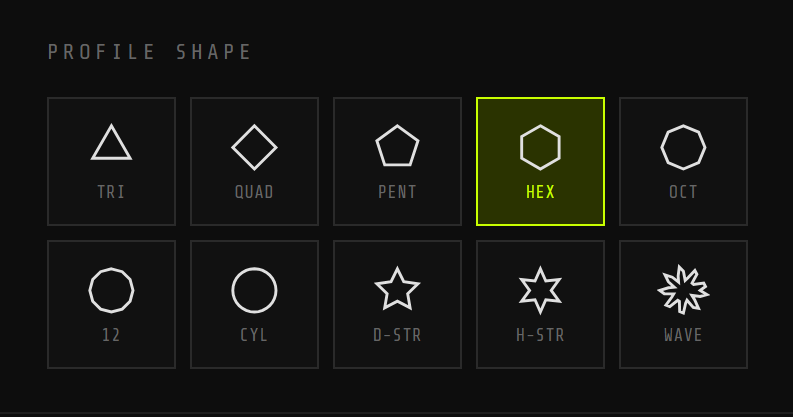
\includegraphics[width=0.9\columnwidth]{ProfileShapes.png}
  \Description{A diagram showcasing various cross-sectional geometric profiles for the knobs, such as triangular, quadrilateral, pentagonal, hexagonal, octagonal, dodecagonal, circular, and star shapes. This demonstrates the visual and tactile shape-coding design options.}
  \caption{Profile shape options including triangle, diamond, pentagon, hexagon, octagon, and star configurations for tactile and visual distinction.}
  \label{fig:profiles}
\end{figure}

\subsection{Mounting, Mutation, and Export Formats}
The customizer supports two mounting strategies: \textbf{Swap-In Mode} (directly replacing the original knob) and \textbf{Slide-Over Mode} (fitting as a non-destructive sleeve over the existing control). To accelerate design, a mutation engine generates variant batches through controlled randomization of unlocked parameters. Mutated designs are rendered in a preview grid (Figure~\ref{fig:output}) to allow rapid physical sampling.

In addition to 3D-printable meshes, ACCESS KNOB features a 2D vector SVG stacking exporter for subtractive fabrication (e.g., laser-cutting or CNC-milling). The exporter slices the 3D model into 2D layer profiles based on user-specified material sheet thickness and laser kerf width (default 0.1 mm). To facilitate quick and accurate manual assembly, the exporter automatically generates two kerf-compensated alignment rods and corresponding slots through all layers, allowing stacked pieces to be precisely aligned and glued.

The tool exports manifold STL meshes, OpenSCAD scripts, 2D SVG layer contours, and JSON/CSV datasets for configuration sharing. This architecture ensures that users with motor impairments retain direct design agency over their own instruments rather than relying on proxies, aligning with the sonic agency framework which asserts the right to shape one's own expressive tools \cite{cavdir2024sonic}.

\begin{figure}[h]
  \centering
  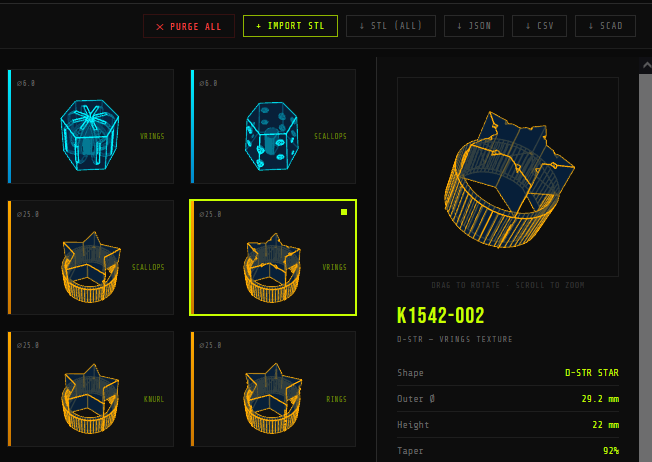
\includegraphics[width=\columnwidth]{OutputDetailsScreen.png}
  \Description{A screenshot of the ACCESS KNOB web interface. The sidebar contains sliders for body dimensions, texture configuration, mounting interface, and mutation settings. The main panel displays a grid of 12 mutated knob variations alongside a detailed inspector panel with 3D preview and numeric parameter listings.}
  \caption{ACCESS KNOB interface showing a batch of 12 generated knob variants with hexagonal profiles. Parameters are displayed for the selected knob (K793-001) including shape, diameter, height, groove geometry, and bore specifications. The mutation engine enables rapid design exploration.}
  \label{fig:output}
\end{figure}

\subsection{Accessibility and Interface Input Options}
A critical consideration in assistive technology design is whether the design tool itself is accessible. A parametric knob customization system that requires fine motor control to operate would perpetuate the very barriers it aims to address. ACCESS KNOB's browser-based architecture supports platform-level accessibility features without custom client-side installation.

\textbf{Apple Voice Control and Switch Control}: macOS and iOS users can operate ACCESS KNOB entirely through voice commands\cite{apple2024voicecontrol} or camera-based facial gestures and head movements\cite{apple2024switchcontrol}. Voice Control enables users to speak commands to navigate, tap buttons, adjust sliders, and trigger exports. Switch Control with camera tracking allows users to control the interface through head movements (left/right gestures) or facial expressions (e.g., smile, raised eyebrows) mapped to interface actions.

\textbf{Google Project Gameface}: Windows and Android users can employ Google's open-source Project Gameface system\cite{google2024gameface,googleblog2023gameface}, which translates head movements and facial gestures into cursor control and click actions. This system operates across any web-based interface, including ACCESS KNOB's parametric controls and mutation engine.

\textbf{Hardware Requirements}: Both Apple and Google solutions require only a standard USB webcam, making assistive input accessible at commodity price points. Higher-end implementations (e.g., Apple TrueDepth cameras on recent devices) provide enhanced facial tracking precision but are not required for functional operation.

\section{Engineering Evaluation and Design Space Analysis}

We evaluate the design space enabled by ACCESS KNOB by analyzing its mechanical advantage, fabrication tolerances, and interface accessibility.

\subsection{Mechanical Torque Advantage}
To quantify how parametric changes reduce the grip force required to actuate a control, we model the mechanical torque $T$ necessary to rotate a potentiometer or rotary switch:
\begin{equation}
T = F \cdot \left(\frac{D}{2}\right) \quad \Longrightarrow \quad F = \frac{2T}{D}
\end{equation}
where $F$ is the applied peripheral finger pinch or grip force, and $D$ is the outer diameter of the knob. Standard synthesizer knobs are relatively small, with diameters typically ranging between $10\text{ mm}$ and $15\text{ mm}$. For a fixed potentiometer resistance torque $T$, increasing the outer diameter to an accessible range ($25\text{--}40\text{ mm}$) substantially decreases the required grip force (Table~\ref{tab:torque_reduction}). For example, replacing a $10\text{ mm}$ original knob with a $30\text{ mm}$ or $40\text{ mm}$ ACCESS KNOB reduces the required force by $66.7\%$ and $75\%$, respectively. This mechanical scaling directly compensates for reduced hand strength without modifying the internal electronic hardware of the instrument.

\begin{table}[h]
\centering
\caption{Comparison of required peripheral force $F$ for different knob diameters $D$ relative to a standard $10\text{ mm}$ control knob ($F_{10}$) for a fixed potentiometer resistance torque $T$.}
\label{tab:torque_reduction}
\begin{tabular}{ccc}
\hline
\textbf{Knob Diameter ($D$)} & \textbf{Required Grip Force ($F$)} & \textbf{Force Reduction} \\ \hline
10\text{ mm} (Standard)  & $F_{10} = \frac{2T}{10}$          & 0\% (Baseline)          \\
15\text{ mm}              & $0.67 \cdot F_{10}$               & 33.3\%                  \\
25\text{ mm} (Medium)    & $0.40 \cdot F_{10}$               & 60.0\%                  \\
32\text{ mm} (Large)     & $0.31 \cdot F_{10}$               & 68.8\%                  \\
40\text{ mm} (Custom)    & $0.25 \cdot F_{10}$               & 75.0\%                  \\ \hline
\end{tabular}
\end{table}

Furthermore, increasing knob height (from standard $12\text{ mm}$ to $25\text{ mm}$ or taller) increases the usable vertical surface area, enabling musicians to employ palm-dragging or side-of-hand shear techniques to actuate the controls.

\subsection{Fabrication Tolerances and Materials}
FDM fabrication with PLA and PETG on a standard Prusa MK3S+ indicates that a bore clearance tolerance $c = 0.2\text{--}0.3\text{ mm}$ is required to accommodate plastic shrinkage and print variances, secured with an M3 set-screw. Rigidity from PLA supports tactile grooves, while PETG's slight elasticity suits slide-over sleeves. Combining a rigid outer shell with a flexible TPU inner sleeve optimizes friction and prevents slippage without scratching original hardware.

For subtractive laser-cutting, stock materials such as acrylic, bamboo, or aluminum composite can be used. Acrylic provides high rigidity and crisp profiles, while bamboo offers unique tactile feedback and superior mechanical vibration-damping characteristics compared to thermoplastic PLA, modifying the physical sensation of the interface during musical performance.

\subsection{Interface Accessibility Conformance}
The browser-based customizer supports keyboard navigation and platform-level hands-free interfaces (Apple Voice/Switch Control, Google Project Gameface) using commodity webcams. For blind or low-vision users, a multimodal interaction loop integrates hidden `aria-live` parameter announcements, oscillator-based parameter sonification (Web Audio API), and short haptic confirmation pulses (`navigator.vibrate()`).

\section{Discussion}

The parametric customizer highlights how browser-based design can support user agency and independence. By operating the tool using standard platform-level accessibility features (such as facial tracking or voice input), users customize control interfaces to match their motor profiles. The non-destructive slide-over sleeves preserve commercial hardware integrity, while tactile shape-coding bridges visual and motor accessibility. Releasing the tool as open-source lowers production costs to cents per knob, though it transfers quality control to user print profiles. Future work will extend the parametric engine to linear faders, drum pads, and foot switches, and will include occupational-therapy-guided clinical trials under an approved IRB protocol to evaluate long-term ergonomic utility.

\section{Acknowledgments}

Anonymized for double-blind review.

\bibliographystyle{ACM-Reference-Format}
\begin{thebibliography}{10}

% Key references from GestoLumina and Sonic Agency papers

\bibitem{hergert2024gestolumina}
[Anonymous]. 2024.
[Anonymized Reference].
In \textit{Proceedings of NIME 2024}.

\bibitem{cavdir2024sonic}
[Anonymous]. 2024.
[Anonymized Reference].
In \textit{Proceedings of ACM SIGACCESS Conference on Computers and Accessibility}.

\bibitem{frid2019accessible}
Emma Frid. 2019.
Accessible Digital Musical Instruments: A Review of Musical Interfaces in Inclusive Music Practice.
\textit{Multimodal Technologies and Interaction} 3, 3 (July 2019), 57.
DOI: 10.3390/mti3030057

\bibitem{mcmillan2023designing}
Andrew McMillan and Fabio Morreale. 2023.
Designing accessible musical instruments by addressing musician-instrument relationships.
\textit{Frontiers in Computer Science} 5 (May 2023), 1153232.
DOI: 10.3389/fcomp.2023.1153232

\bibitem{mccloskey2015accessibility}
Brendan McCloskey, Brian Bridges, and Frank Lyons. 2015.
Accessibility And Dimensionalty: Enhanced Real-Time Creative Independence For Digital Musicians With Quadriplegic Cerebral Palsy.
In \textit{Proceedings of NIME 2015}.
DOI: 10.5281/ZENODO.1179132

\bibitem{payne2020eye}
William C Payne, Ann Paradiso, and Shaun Kane. 2020.
Cyclops: Designing an eye-controlled instrument for accessibility and flexible use.
In \textit{Proceedings of NIME 2020}.
DOI: 10.5281/ZENODO.4813204

\bibitem{tandon2023parametric}
Mixuan Li and Leila Aflatoony. 2023.
A Parametric Design Tool to Support Customized Adaptations of Assistive Technologies for People with Hand Impairments.
In \textit{Proceedings of the 25th International ACM SIGACCESS Conference on Computers and Accessibility (ASSETS '23)}.
ACM, Article 32, 1--15.
DOI: 10.1145/3597638.3614492

\bibitem{santos2023parametric}
Rune Thorsen, Denise Cugnod, Marina Ramella, Rosa Converti, and Maurizio Ferrarin. 2024.
A parametric 3D printed assistive device for people with cerebral palsy -- assessment of outcomes and comparison with a commercial counterpart.
\textit{Assistive Technology} 36, 1 (2024), 16--21.
DOI: 10.1080/10400435.2023.2202696

\bibitem{hofmann2020living}
Megan Hofmann, Devva Kasnitz, Jennifer Mankoff, and Cynthia L Bennett. 2020.
Living Disability Theory: Reflections on Access, Research, and Design.
In \textit{Proceedings of the 22nd International ACM SIGACCESS Conference on Computers and Accessibility}.
ACM, 1--13.
DOI: 10.1145/3373625.3416996

\bibitem{desai20153dprinting}
Ruta Desai, Huaishu Peng, Stelian Coros, James McCann, and Scott E. Hudson. 2015.
3D Printing Pneumatic Device Controls with Variable Activation Force Capabilities.
In \textit{Proceedings of the 33rd Annual ACM Conference on Human Factors in Computing Systems (CHI '15)}.
ACM, 3799--3808.
DOI: 10.1145/2702123.2702516

\bibitem{holland2020expanding}
Quinn D Jarvis Holland, Crystal Quartez, Francisco Botello, and Nathan Gammill. 2020.
Expanding Access to Music Technology: Rapid Prototyping Accessible Instrument Solutions For Musicians With Intellectual Disabilities.
In \textit{Proceedings of NIME 2020}.
DOI: 10.5281/ZENODO.4813286

\bibitem{manenti2024accessibility}
Francesco Manenti and Francesco Ardan Dal Rì. 2024.
Accessibility of Graphic Scores: Design and Exploration of Tactile Supports for Blind People.
In \textit{Proceedings of NIME 2024}.
DOI: 10.5281/ZENODO.13904941

\bibitem{cavdir2022touch}
Doga Cavdir. 2022.
Touch, Listen, (Re)Act: Co-designing Vibrotactile Wearable Instruments for Deaf and Hard of Hearing.
In \textit{Proceedings of NIME 2022}.
DOI: 10.21428/92fbeb44.b24043e8

\bibitem{cavdir2020felt}
Doga Cavdir and Ge Wang. 2020.
Felt Sound: A Shared Musical Experience for the Deaf and Hard of Hearing.
In \textit{Proceedings of NIME 2020}.
DOI: 10.5281/ZENODO.4813305

\bibitem{wink2018balance}
M. E. Wink. 2018.
Current balance levels in deaf and hearing impaired children.
Master's thesis. University of Tennessee, Knoxville.

\bibitem{treviranus2014}
Jutta Treviranus. 2014.
The Value of the Curb Cut Effect.
\textit{Slaw (Co-operative Legal Journal)}.
Retrieved January 21, 2014 from \url{http://www.slaw.ca/2014/01/21/the-value-of-the-curb-cut-effect/}

\bibitem{apple2024voicecontrol}
Apple Inc. 2024.
Use Voice Control on your iPhone, iPad, or iPod touch.
Apple Support.
Retrieved May 20, 2025 from \url{https://support.apple.com/en-us/111778}

\bibitem{apple2024switchcontrol}
Apple Inc. 2024.
Use Switch Control to navigate your iPhone, iPad, or iPod touch.
Apple Support.
Retrieved May 20, 2025 from \url{https://support.apple.com/en-us/119835}

\bibitem{google2024gameface}
Google LLC. 2024.
Project Gameface.
GitHub repository.
Retrieved May 20, 2025 from \url{https://github.com/google/project-gameface}

\bibitem{googleblog2023gameface}
Google LLC. 2023.
Google Project Gameface: A new hands-free AI-powered gaming mouse.
The Keyword (Google Blog).
Retrieved May 20, 2025 from \url{https://blog.google/innovation-and-ai/products/google-project-gameface/}

% Additional references on Universal Design, synthesizer accessibility, etc.
% TODO: Add 5-10 more references from web search results on:
% - Universal Design principles in music/HCI
% - Occupational therapy for grip strength
% - Generative design for assistive technology
% - DHH musicianship research
% - 3D printing materials for tactile devices

\end{thebibliography}

\end{document}
